\documentclass[a4paper]{article}
\usepackage[utf8]{inputenc}
\usepackage[german]{babel}
\usepackage{amsmath}
\usepackage{amsfonts}
\usepackage{amssymb}
\usepackage{graphicx}

\author{Merlin Koglin, Timon Vosberg, Merlin Steuer}
\date{Abgabe: 23. Januar 2016}
\title{Lösungen zu Aufgabenblatt 11}


\begin{document}
\maketitle
\tableofcontents

\newpage

\section{Jacobi}
\subsection{Start}
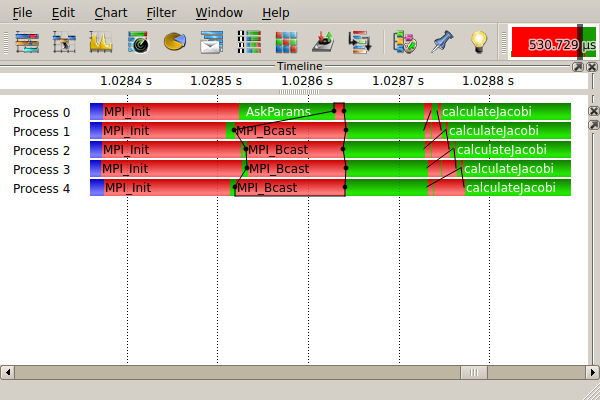
\includegraphics[scale=0.9]{img/ja_5_4_start.png}

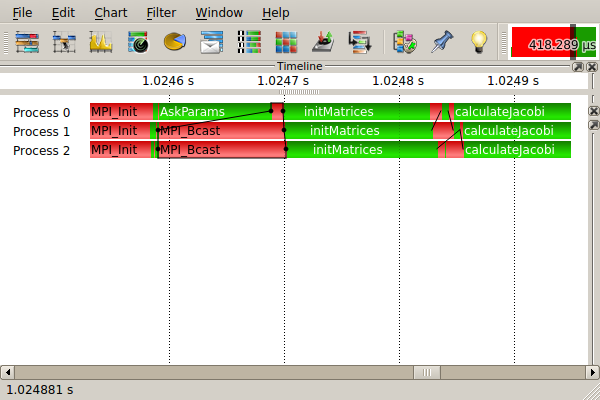
\includegraphics[scale=0.9]{img/ja_3_2_start.png}

Man sieht schön, wie nach dem Abfragen der Eingabeparameter alle Prozesse gleichzeitig Speicher für die Matrizen reservieren und dann etwas zeitversetzt starten, nachdem alle Zeilendaten mit Vorgängern bzw. Nachfolgern ausgetauscht worden sind.
\subsection{Synchronisation}
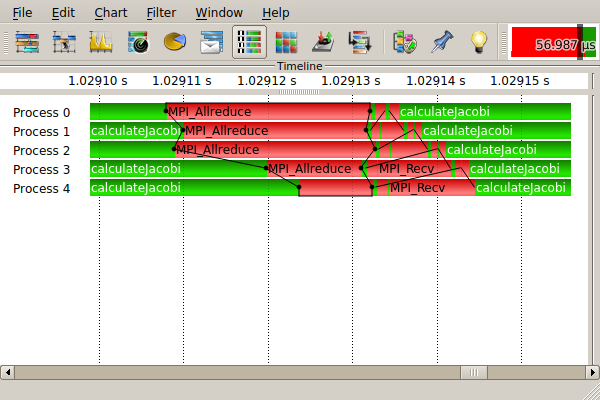
\includegraphics[scale=0.9]{img/ja_5_4_synchro.png}

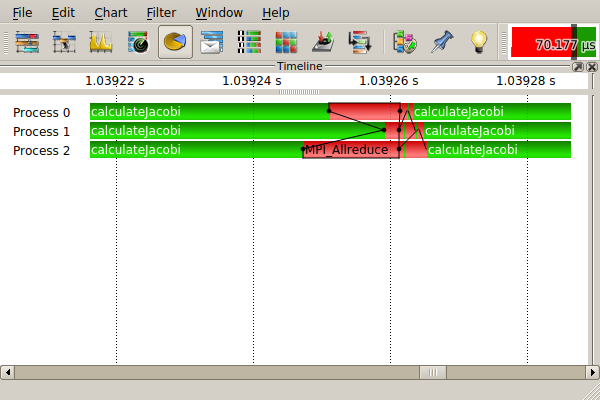
\includegraphics[scale=0.9]{img/ja_3_2_synchro.png}

Man erwartet, dass alle Prozesse gleichzeitig mit dem Berechnen einer Iteration fertig sind. Dies ist jedoch nicht der Fall, entsprechend muss der schnellste Prozess relativ lange auf das Allreduce der residuums warten. Sobald alle Prozesse geantwortet haben beginnt wieder der Zeilenaustausch. Bis auf die kleinen Abweichungen geschieht auch hier alles wie erwartet.
\subsection{Ende}
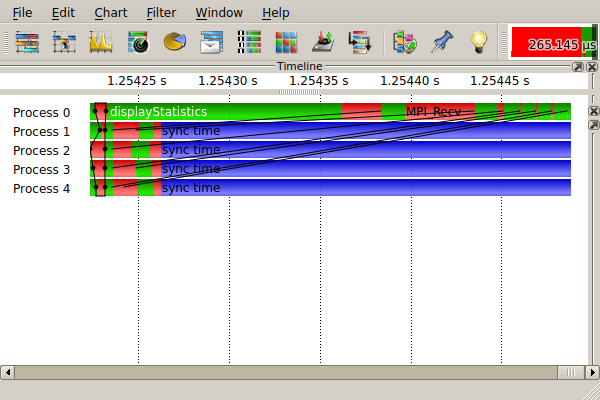
\includegraphics[scale=0.9]{img/ja_5_4_end.png}

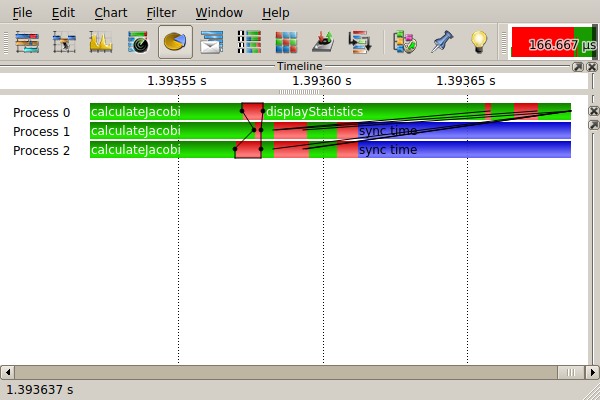
\includegraphics[scale=0.9]{img/ja_3_2_end.png}

Ganz zum Schluss passiert beim Jacobi noch eine letzte Allreduce, nach der der Abbruch entschieden wird. Alle Prozesse senden ihre Daten zur Anzeige an den Master-Prozess.
\section{Gauß-Seidel}
\subsection{Start}
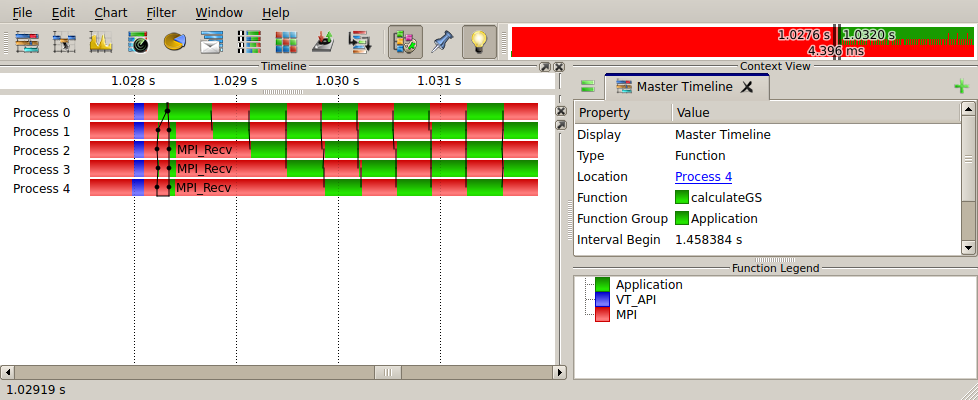
\includegraphics[scale=0.85]{img/gs_5_4_start.png}

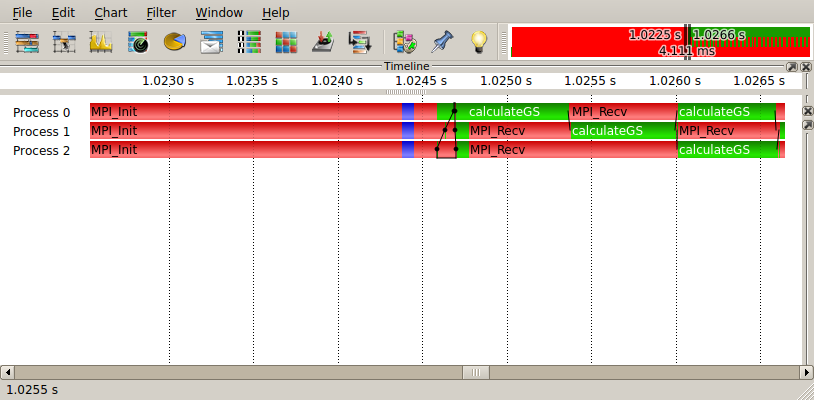
\includegraphics[scale=0.7]{img/gs_3_2_start.png}

Auch hier beginnen alle Prozesse gleichzeitig mit dem Allokieren von Speicher für die Matrizen. Danach sieht man hier sehr schön, wie die Pipeline aufgebaut wird.

Diese Bilder erklären sehr eindrücklich, wieso unsere Gauß-Seidel-Implementation immer etwa doppelt so lange gebraucht hat wie die Jacobi-Implementation. Die Daten der ersten Zeile des Nachfolgeprozesses werden erst empfangen, sobald dieser die komplette Iteration berechnet hat. Damit kann ein Prozess niemals parallel zu seinen direkten Nachbarn berechnen. Abhilfe würde hier schaffen, mittels eines ISend-Befehls die erste Zeile direkt an den Vorgänger zu schicken, sobald diese fertig berechnet ist.
\subsection{Synchronisation}
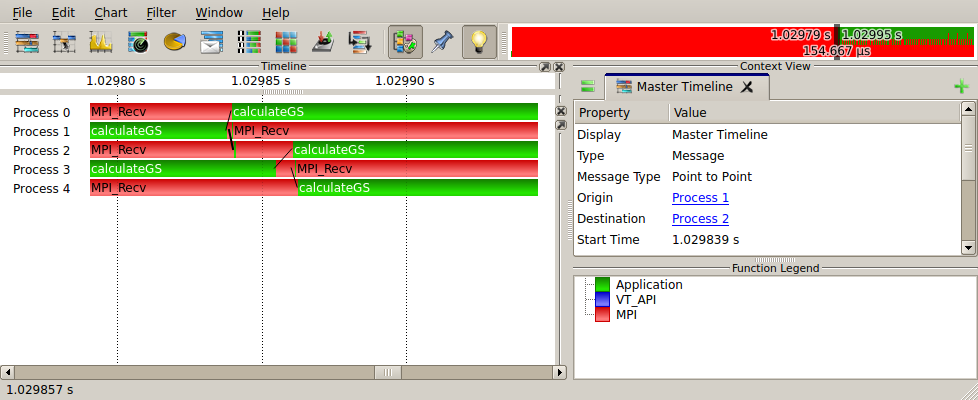
\includegraphics[scale=0.85]{img/gs_5_4_synchro.png}

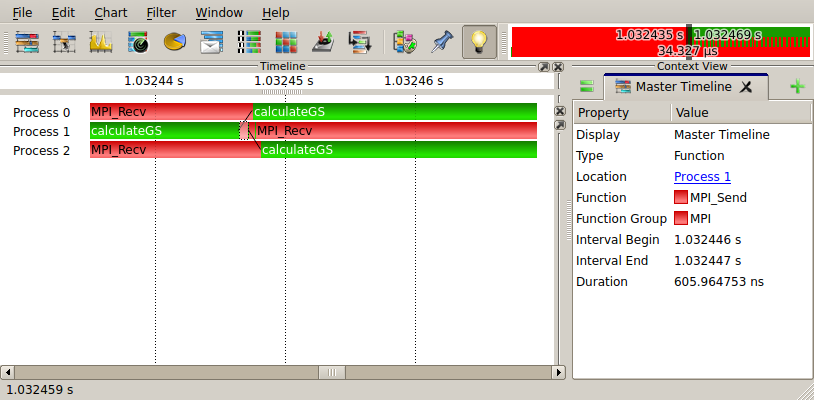
\includegraphics[scale=0.85]{img/gs_3_2_synchro.png}

Dies setzt sich hier natürlich fort, man sieht wie die erste Zeile des Datensatzes eines Prozesses an den Vorgänger geschickt wird und direkt daraufhin der Vorgänger los rechnet. Danach wird die letzte Zeile zum Nachfolger geschickt, damit dieser die nächstem Iteration rechnen kann. Der Gegenseitige Ausschluss eines Prozesses zu seinen Nachbarn ist hier noch ein mal deutlich visualisiert.
\subsection{Ende}
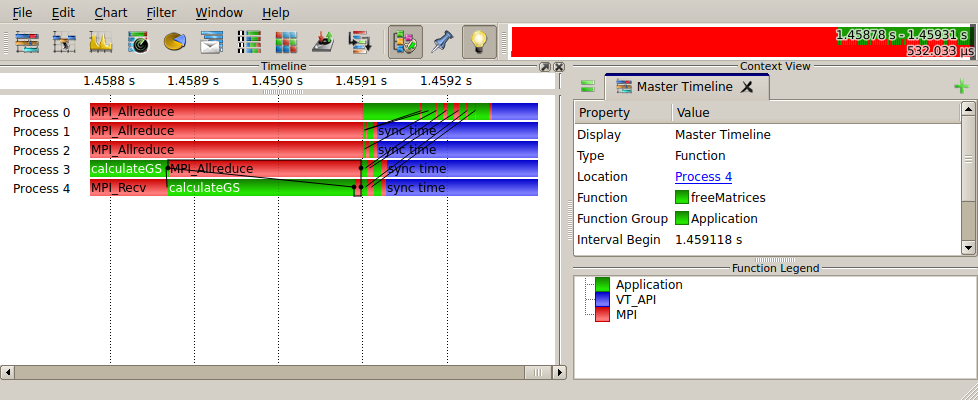
\includegraphics[scale=0.9]{img/gs_5_4_end1.png}

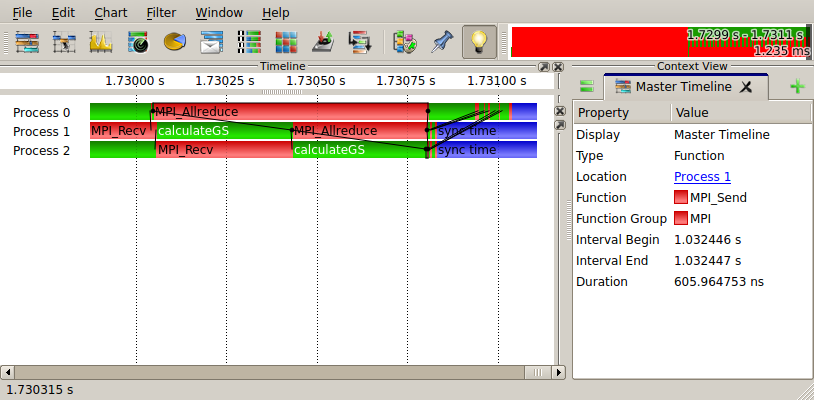
\includegraphics[scale=0.9]{img/gs_3_2_end.png}

Gut zu sehen ist hier, dass alle Prozesse auf den letzten warten müssen, um die Allreduce-Funktion zu beenden und außerdem die Statistiken wieder verteilt auszugeben. Ansonsten ist der Ablauf wie erwartet.
\end{document}